\section{Paper Reading: Non-Local}


\begin{frame}{Non-local Neural Networks (CVPR 2018)\cite{NonLocal2018}}
    \begin{itemize}
        \item \textbf{Title:}Non-local Neural Networks
        \item \textbf{Author:} Xiaolong Wang, Ross Girshick, Abhinav Gupta, Kaiming He\footnote{Carnegie Mellon University, Facebook AI Research}
        \item \textbf{Code:} https://github.com/facebookresearch/video-nonlocal-net
    \end{itemize}
\end{frame}


\begin{frame}{Non-local}
    \textbf{Non-local}
    \begin{equation}
        y_i=\frac{1}{C(x)}\sum_{\forall j}f(x_i,x_j)g(x_j)
    \end{equation}
    $C(x)$是归一化系数,$f(x_i,x_j)$用来计算输入信号在$x_j$位置与$x_i$的相似性/相关性,并且对$g(x_j)$进行加权,$g(x_j)$计算输入信号在$j$位置的特征值。
    \begin{itemize}
        \item \textbf{Gaussian.} $f(x_i,x_j)=e^{x_i^T x_j}$, $C(x)=\sum_{\forall j}f(x_i,x_j)$
        \item \textbf{Embedded Gaussian.} $f(x_i,x_j)=e^{\theta(x_i)^T \Phi(x_j)}$, $C(x)=\sum_{\forall j}f(x_i,x_j)$
        \item \textbf{Dot product.} $f(x_i,x_j)=\theta(x_i)^T \Phi(x_j)$, $C(x)=N$
        \item \textbf{Concatenation.} $f(x_i,x_j)=ReLU(w_f^T [\theta(x_i),\Phi(x_j)])$, $C(x)=N$
    \end{itemize}
\end{frame}

\begin{frame}{Non-local}
    \begin{multicols}{2}
        \begin{figure}
            \centering
            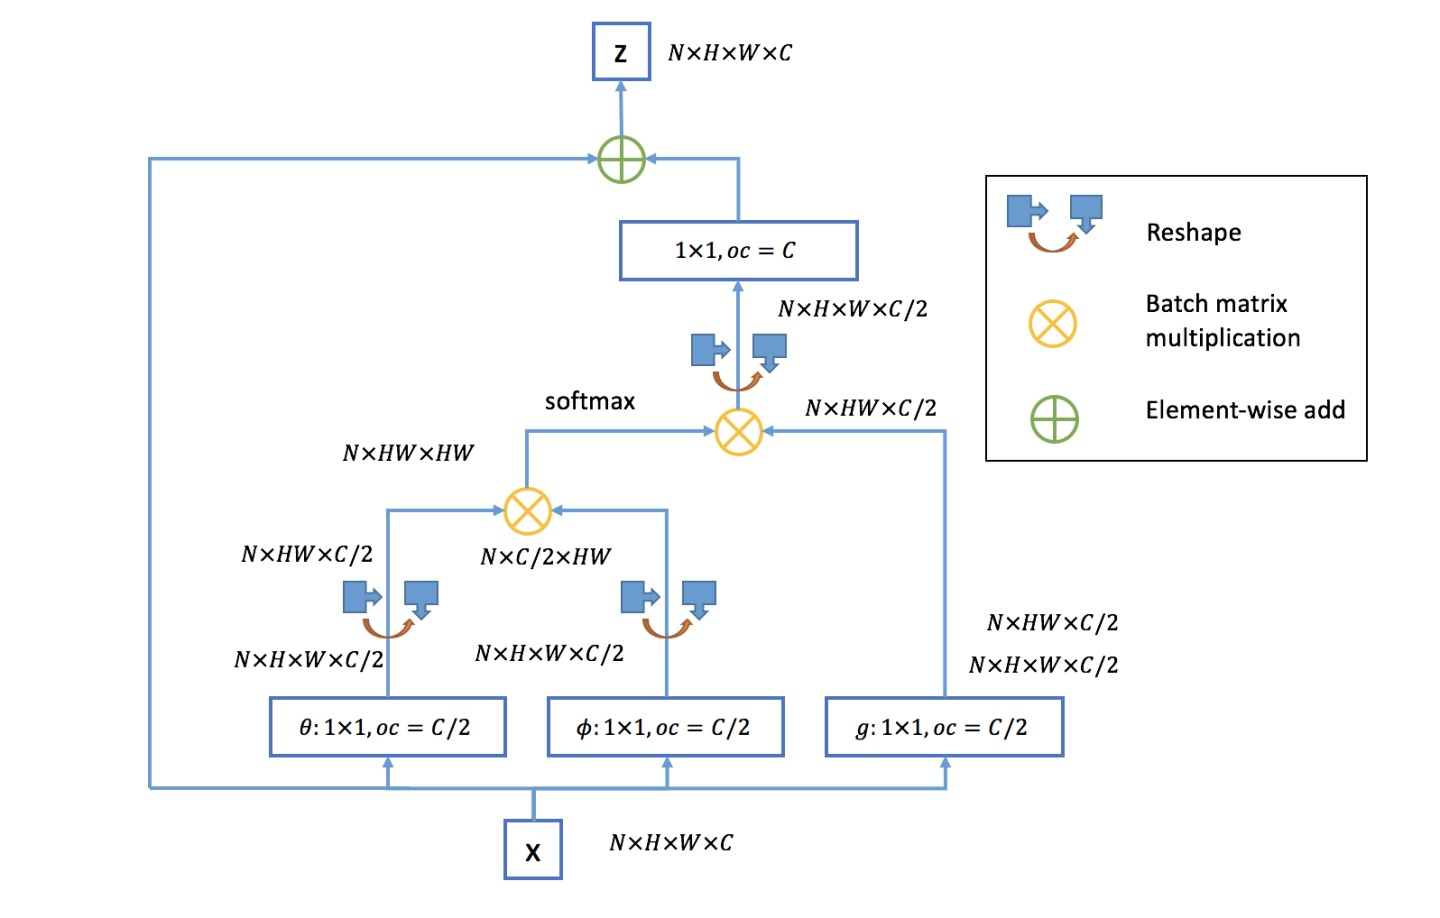
\includegraphics[width=0.6\textwidth]{docs/paperReading/Non-local/non-local.jpg}
        \end{figure}
        

        \textbf{Non-local Block}
        \begin{equation}
            z_i=W_z y_i+x_i
        \end{equation}
        \hspace*{\fill}
        \hspace*{\fill}
        \hspace*{\fill}
        \begin{equation}
            y_i=Softmax(\theta(x_i)^T \Phi(x_j))g(x_j)
        \end{equation}
        $\theta(x_i)$表示局部,$\Phi(x_i)$是

    \end{multicols}
\end{frame}

\begin{frame}{Experiment in Kinetics Dataset}    
    \begin{multicols}{2}       
        \begin{figure}
            \centering
            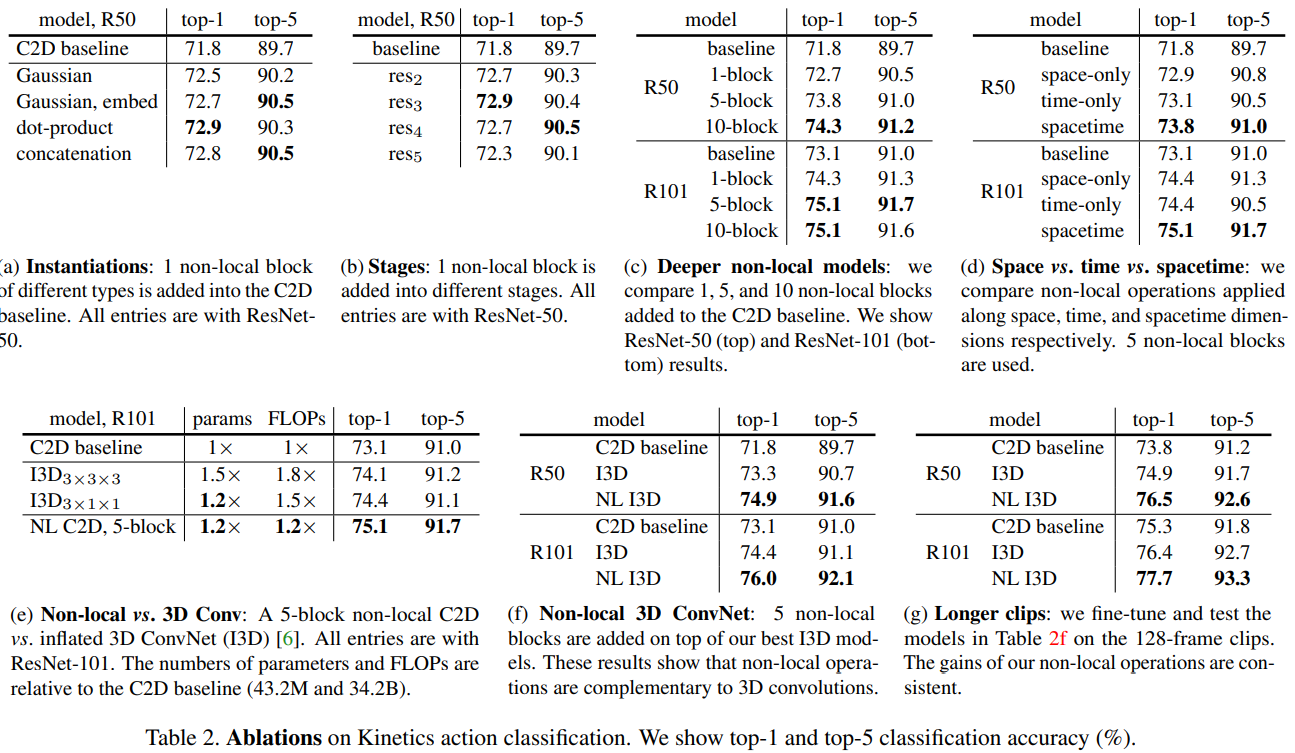
\includegraphics[width=0.54\textwidth]{docs/paperReading/Non-local/exp.png}
        \end{figure}

        \begin{scriptsize}
            Kinetics Dataset: 行为识别 benchmark
            \begin{itemize}
                \item (a) 四种相似度计算模型$f$对比
                \item (b) non-local加在ResNet-50不同的stage下。在stage3,4添加提升acc较大
                \item (c) 在ResNet-50和ResNet-101中添加不同数量的non-local block。添加数量越多,效果越好
                \item (d) 在
                \item (e) 与3D Conv在参数量、计算量、acc进行对比
                \item (f) 在3D Conv加入non-local模块
            \end{itemize}
        \end{scriptsize}
    \end{multicols}
\end{frame}

\begin{frame}{Experiment}    
    \begin{figure}
        \centering
        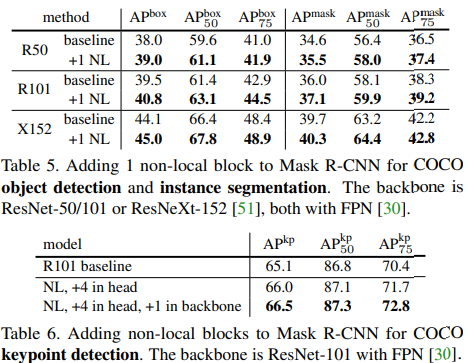
\includegraphics[width=0.5\textwidth]{docs/paperReading/Non-local/assignment.png}
    \end{figure}

    \begin{scriptsize}
        基于COCO数据集,Non-local应用在object detection, instance segmentation, keypoint detection等任务上
    \end{scriptsize}
\end{frame}


\begin{frame}{Experiment(*)}
    \begin{scriptsize}
        将Non-local block添加到网络中,分别是:
        \begin{itemize}
            \item \textbf{ResNet-50}
            \item \textbf{ResNet-50 Non-local layer-1}: 在 $layer1$ 后添加 $1$ 个Non-Local Block
            \item \textbf{ResNet-50 Non-local layer-2}: 在 $layer2$ 后添加 $1$ 个Non-Local Block
            \item \textbf{ResNet-50 Non-local layer-3}: 在 $layer3$ 后添加 $1$ 个Non-Local Block
            \item \textbf{ResNet-50 Non-local layer-4}: 在 $layer4$ 后添加 $1$ 个Non-Local Block
            \item \textbf{ResNet-50 Non-local 5-block}: 在 $layer3$ 后添加 $3$ 个、在 $layer4$ 后添加 $2$ 个,共5个Non-Local Block
            \item \textbf{ResNet-50 Non-local 10-block}: 在 $layer3$ 后添加 $5$ 个、在 $layer4$ 后添加 $5$ 个,共10个Non-Local Block
        \end{itemize}

        \begin{table}
            \centering
            \begin{tabular}{ll}
                arch & test accuracy \\
                resnet50 & 0.93750 \\
                resnet50_nonlocal_layer1 & 0.93300 \\
                resnet50_nonlocal_layer2 & 0.94000 \\
                resnet50_nonlocal_layer3 & \textbf{0.94450} \\
                resnet50_nonlocal_layer4 & 0.93750 \\
                resnet50_nonlocal_5block & 0.91550 \\
                resnet50_nonlocal_10block & 0.89050
            \end{tabular}
            \end{table

    \end{scriptsize}
\end{frame}

\begin{frame}{Experiment(*)}
    \begin{multicols}{2}
    \begin{figure}
        \centering
        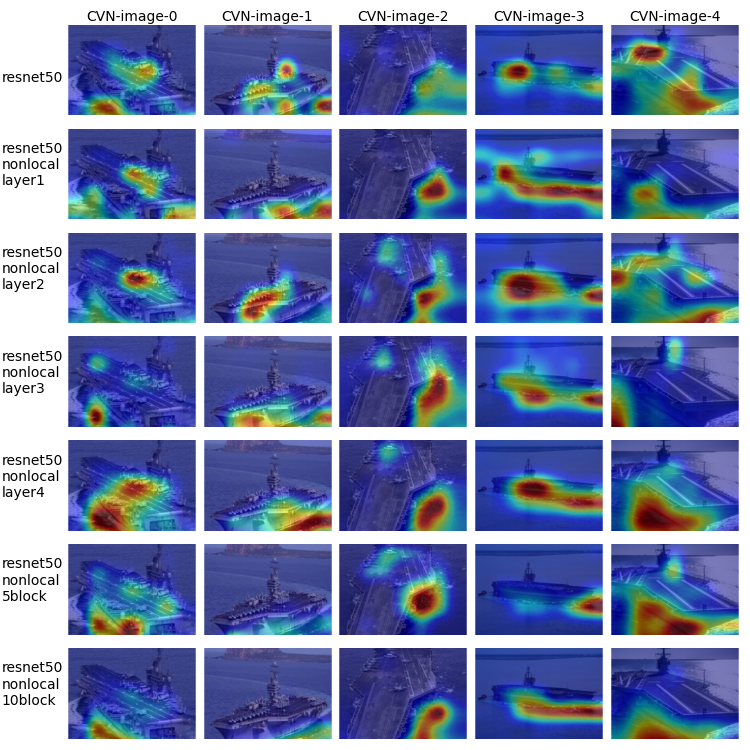
\includegraphics[width=0.45\textwidth]{docs/paperReading/Non-local/exp/CVN.png}
        \caption{class:CVN}
    \end{figure}

    \begin{scriptsize}
        图中从上至下,分别是:

        \begin{tiny}
            \textbf{ResNet-50}

            \textbf{ResNet-50 Non-local layer-1}: 在 $layer1$ 后添加 $1$ 个Non-Local Block

            \textbf{ResNet-50 Non-local layer-2}: 在 $layer2$ 后添加 $1$ 个Non-Local Block

            \textbf{ResNet-50 Non-local layer-3}: 在 $layer3$ 后添加 $1$ 个Non-Local Block
            
            \textbf{ResNet-50 Non-local layer-4}: 在 $layer4$ 后添加 $1$ 个Non-Local Block
            
            \textbf{ResNet-50 Non-local 5-block}: 在 $layer3$ 后添加 $3$ 个、在 $layer4$ 后添加 $2$ 个,共5个Non-Local Block
            
            \textbf{ResNet-50 Non-local 10-block}: 在 $layer3$ 后添加 $5$ 个、在 $layer4$ 后添加 $5$ 个,共10个Non-Local Block
        \end{tiny}

        类别: CVN 
    \end{scriptsize}
\end{multicols}
\end{frame}

\begin{frame}{Experiment(*)}
    \begin{multicols}{2}
    \begin{figure}
        \centering
        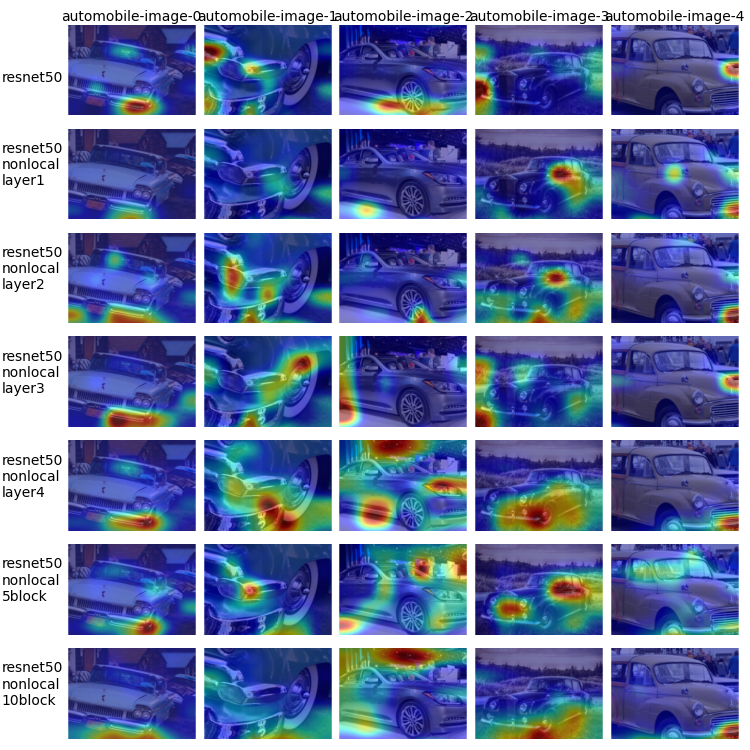
\includegraphics[width=0.45\textwidth]{docs/paperReading/Non-local/exp/automobile.png}
        \caption{class:automobile}
    \end{figure}

    \begin{scriptsize}
        图中从上至下,分别是:

        \begin{tiny}
            \textbf{ResNet-50}

            \textbf{ResNet-50 Non-local layer-1}: 在 $layer1$ 后添加 $1$ 个Non-Local Block

            \textbf{ResNet-50 Non-local layer-2}: 在 $layer2$ 后添加 $1$ 个Non-Local Block

            \textbf{ResNet-50 Non-local layer-3}: 在 $layer3$ 后添加 $1$ 个Non-Local Block
            
            \textbf{ResNet-50 Non-local layer-4}: 在 $layer4$ 后添加 $1$ 个Non-Local Block
            
            \textbf{ResNet-50 Non-local 5-block}: 在 $layer3$ 后添加 $3$ 个、在 $layer4$ 后添加 $2$ 个,共5个Non-Local Block
            
            \textbf{ResNet-50 Non-local 10-block}: 在 $layer3$ 后添加 $5$ 个、在 $layer4$ 后添加 $5$ 个,共10个Non-Local Block
        \end{tiny}

        类别: automobile 
    \end{scriptsize}
\end{multicols}
\end{frame}

\begin{frame}{Experiment(*)}
    \begin{multicols}{2}
    \begin{figure}
        \centering
        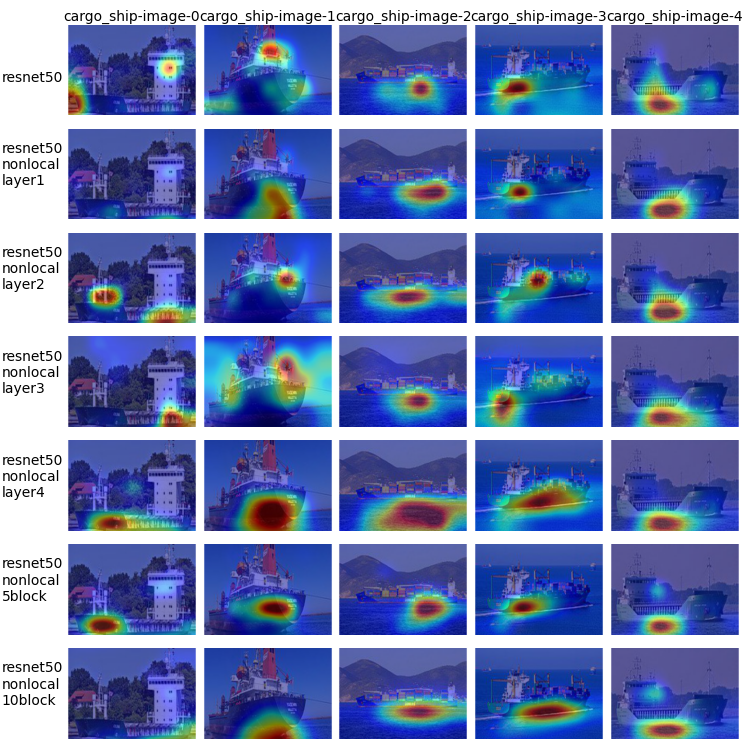
\includegraphics[width=0.45\textwidth]{docs/paperReading/Non-local/exp/cargo_ship.png}
        \caption{class:cargo_ship}
    \end{figure}

    \begin{scriptsize}
        图中从上至下,分别是:

        \begin{tiny}
            \textbf{ResNet-50}

            \textbf{ResNet-50 Non-local layer-1}: 在 $layer1$ 后添加 $1$ 个Non-Local Block

            \textbf{ResNet-50 Non-local layer-2}: 在 $layer2$ 后添加 $1$ 个Non-Local Block

            \textbf{ResNet-50 Non-local layer-3}: 在 $layer3$ 后添加 $1$ 个Non-Local Block
            
            \textbf{ResNet-50 Non-local layer-4}: 在 $layer4$ 后添加 $1$ 个Non-Local Block
            
            \textbf{ResNet-50 Non-local 5-block}: 在 $layer3$ 后添加 $3$ 个、在 $layer4$ 后添加 $2$ 个,共5个Non-Local Block
            
            \textbf{ResNet-50 Non-local 10-block}: 在 $layer3$ 后添加 $5$ 个、在 $layer4$ 后添加 $5$ 个,共10个Non-Local Block
        \end{tiny}

        类别: cargo_ship 
    \end{scriptsize}
\end{multicols}
\end{frame}

